\documentclass[11pt,a4paper,french]{article}

\usepackage[utf8]{inputenc}
\usepackage[T1]{fontenc}
\usepackage{lmodern}
\usepackage{multirow}
\usepackage[french]{babel}
\usepackage[version=3]{mhchem}
\usepackage[Gray,squaren]{SIunits}
\usepackage{color}
\usepackage{chemfig}
\usepackage{numprint}
\usepackage{hyperref}

\pagestyle{plain}

\title{Synthèse de Chimie Q2}
\author{Benoît Legat \and Lucas Nyssens \and Laurent Opsomer}

\renewcommand{\textbf}[1]{\begingroup\bfseries\mathversion{bold}#1\endgroup}

\newcommand\sorb{\mathrm{s}}
\newcommand\porb{\mathrm{p}}
\newcommand\dorb{\mathrm{d}}
\newcommand\gaz{_{(g)}}
\newcommand\solid{_{(s)}}
\newcommand\liquid{_{(l)}}
\newcommand\debye{\mathrm{D}}
\newcommand\calo{\mathrm{cal}}
\newcommand\atm{\mathrm{atm}}
\newcommand\ccal{C_\mathrm{cal}}
\newcommand\qrev{\ensuremath{q_{\mathrm{rév}}}}
\newcommand\kc{\ensuremath{K_{\mathrm{c}}}}
\newcommand\kp{\ensuremath{K_{\mathrm{p}}}}
\newcommand\keq{\ensuremath{K_{\mathrm{éq}}}}
\newcommand\eqdef{\stackrel{\Delta}{=}}

\begin{document}
\maketitle

\part{Notions de base}

\paragraph{Propriétés de la matière}
\begin{itemize}
	\item Propriétés \textbf{extensives}: Dépendent de la quantité de matière (Ex: Masse, énergie,...).
	\item Propriétés \textbf{intensives}: Ne dépendent pas de la quantité de matière (Ex: Température, pression,...).
\end{itemize}

\paragraph{A. Lavoisier}
\begin{enumerate}
	\item Loi de conservation de la masse: ``Dans un conteneur étanche, ni création, ni perte de matière''.
	\item Loi des compositions définies: ``Dans un composé pur, les éléments sont toujours présents dans des proportions définies''.
\end{enumerate}

\paragraph{Chaleur de réaction:}
\'Energie de réaction: énergie absorbée par le système (par convention)
$$\Delta E = E_{\textrm{produits}}-E_{\textrm{réactifs}}$$

Si réaction endothermique: absorption d'énergie $\Rightarrow \Delta E > 0$

Si réaction exothermique: dégagement d'énergie $\Rightarrow  \Delta E < 0$

\part{Atomistique}

%\subsection{\'Electrons de coeur}
%Les électrons de coeur sont tous les électrons sauf les électrons de valences.

%\paragraph{Exemple}
%$\ce{Zn}$ de composition $[\ce{Ar}]3\dorb^{10}4\sorb^{2}$
%a 28 électrons de coeur car $\ce{Ar}$ a 18 électrons
%et la derniére couche est $n=4$,
%donc $3\dorb^{10}$ n'y est pas et peut être compté.
%On peut aussi dire qu'il en a 18 en prenant une valence de 12.

\paragraph{Nombres atomiques et de masse}

\emph{$^{A}_{Z}X$}
\begin{itemize}
	\item $Z$: nombre atomique = nombre de protons dans le noyau = nombre d'électrons
	\item $A$: nombre de masse = nombre de protons et de neutrons dans le noyau (car masse $e^{-}$ négligeable)
	\item \# neutrons = $A-Z$
	\item Isotopes: même nombre de protons, nombre de neutrons différent.
\end{itemize}

\section{Rayonnement électromagnétique}

La lumière, les ondes radios,... sont des formes de rayonnements électromagnétiques constitués d'un champ électrique oscillant et d'un champ magnétique oscillant $\Rightarrow$ transportent de l'énergie.

Caractéristiques:
\begin{itemize}
	\item Longueur d'onde $\lambda$ (\meter)
	\item Fréquence $\nu$ (\hertz)
	\item Vitesse (de la lumière) $c$ (\meter\per\second)
\end{itemize}

On sait que
\[ c = \lambda \nu \]

Si le rayonnement est dans le vide
\[ c = c_0 \]

Un rayonnement électromagnétique ne peut transmettre de l'énergie que par {\it quanta}, qui est l'énergie transmise par un photon et qui vaut
\[ E = h\nu \]

L'énergie transmise par électron passant d'une couche à une distance $n_i$ à un couche à une distance $n_f$ vaut
\[ \Delta E = h\nu = \frac{hc}{\lambda} = R_y \left( \frac{1}{n_f^2} - \frac{1}{n_i^2} \right) \]
où $R_y = hc R_\infty = \numprint[\joule]{2,178e-18}$ est la constante de Rydberg.

On a aussi, la longueur d'onde de Broglie
\[ \lambda = \frac{h}{m\nu} \]

Les électrons (et la matière en général) ont à la fois un caractère ondulatoire et un caractère corpusculaire.


\section{Fonction d'onde}

Dualité onde-particule $\Rightarrow$ les électrons ne tournent pas autour du noyau selon une trajectoire définie.

$\Rightarrow$ Fonction d'onde $\psi$ (solutions équation de Schrödinger)\\

Max Born: $\psi^2 = $ densité de probabilité de présence de la particule (probabilité de présence/volume).

Les \textbf{orbitales atomiques} sont les fonctions d'onde des électrons dans les atomes.

\section{Nombres quantiques}

Un électron dans un atome voyage toujours sur une orbitale.
Deux électrons ne peuvent pas être tous les deux sur la même orbitale.
Les orbitales peuvent être décrites par 4 paramètres.

\subsection{Le nombre quantique principal}
L'électron se déplace dans son orbite le long d'une sinusoïde, $n$ détermine le nombre de période qu'il fait par tour.
Il faut que la circonférence de l'orbite soit un multiple de $\lambda$.
D'où
\[ n\lambda = 2\pi r \]

Par la longueur d'onde de Broglie
\[ n \frac{h}{2\pi} = m \nu r \]

$n$ détermine donc aussi le rayon de l'orbitale et son énergie.
On voit que $n$ est proportionnel au rayon de l'orbitale.
$n$ peut prendre les valeurs $1, 2, \ldots$

$n$ détermine la couche de l'orbitale.
%La valeur de $n$ peut aussi être représenté par la période correspondante
% NOT SURE
%\begin{center}
%\begin{tabular}{c|ccccc}
%	$n$ & 1 & 2 & 3 & 4 & \multirow{2}{*}{$\cdots$}\\
%	\cline{1-5}
%	Période & K & L & M & N
%\end{tabular}
%\end{center}

\subsection{Le nombre quantique secondaire}
$l$ détermine la forme de l'orbitale.
Il y a exactement $n$ formes possible pour une orbitale de nombre quantique $n$.

{\bf La numérotation se fait}, comme en informatique, {\bf à partir de $0$}.
Pour une orbitale de nombre quantique $n$, $l$ peut prendre les valeurs $0, 1, \ldots, n-1$

$l$ détermine la sous-couche de l'orbitale.

La valeur de $l$ peut aussi être représenté par une lettre minuscule

\begin{center}
	\begin{tabular}{c|cccccc}
		$l$ & 0 & 1 & 2 & 3 & 4 & \multirow{2}{*}{$\cdots$}\\
		\cline{1-6}
		Lettre & s & p & d & f & g\\
		Origine & {\bf s}harp & {\bf p}rincipal & {\bf d}iffuse & {\bf f}ondamental
	\end{tabular}
\end{center}

\subsection{Le nombre quantique magnétique}
$m_l$ détermine l'orientation relative de l'orbitale par rapport aux autres orbitales de sa sous-couche.
Il y a exactement $2l + 1$ orientation possible pour une orbitale de nombre quantique $l$.
Pour une orbitale de nombre quantique $l$, $m_l$ peut prendre les valeurs $-l, \ldots, -1,  0, 1, \ldots, l$

\subsection{Le nombre quantique de spin}
$m_s$ détermine le sens dans lequel l'électron se déplace.
$m_s$ peut prendre les valeurs $-\frac{1}{2}$ et $\frac{1}{2}$.

La valeur de $m_s$ peut aussi être représenté par l'orientation du moment magnétique de l'électron dans l'orbitale correspondante

\begin{center}
	\begin{tabular}{c|cc}
		$m_s$ & $-\frac{1}{2}$ & $\frac{1}{2}$\\
		\hline
		Moment magnétique & up & down
	\end{tabular}
\end{center}

% E ^
%  n v
%  r v
%  Z ^
%  Ecrantage v
% s > p > d > f

\section{Structure électronique de l'hydrogène}
\begin{itemize}
	\item \'Etat fondamental: l'$e^-$ occupe une orbitale 1s
	\item Si l'$e^-$ acquiert assez d'énergie, il peut atteindre d'autres couches: n=2 (2s ou une des trois sous-couches 2p), n=3,4... et s'il acquiert suffisamment d'énergie $\rightarrow$ quitte l'atome.
\end{itemize}

Dans le cas de l'atome d'hydrogène, l'énergie est donc uniquement fonction du nombre quantique $n$.

\section{Atomes polyélectroniques}
\begin{itemize}
	\item \'Ecrantage: les électrons se repoussent les uns les autres $\Rightarrow$ moins attirés par le noyau.
	\item Effet de pénétration des $e^-$: un $e^-$ \textit{s} de n'importe quelle couche peut se trouver près du noyau $\rightarrow$ il peut pénétrer à travers les couches internes.
		Un $e^-$ \textit{p} pénètre beaucoup moins (sa fonction d'onde s'annule sur le noyau) $\Rightarrow$ charge nucléaire effective inférieure à celle que subit l'$e^-$\textit{s}.
	\item \'Energie fonction de $n$ et de $l$.
\end{itemize}
$\Rightarrow$ Ordre des énergies des orbitale: $s<p<d<f<...$

\section{Remplissage des orbitales}
\begin{itemize}
	\item Règle de Klechkowsky: remplissage des orbitales par ordre croissant d'énergie
	\item Principe d'exclusion de Pauli: Deux électrons ne peuvent pas occuper un même état quantique dans 1 atome $\Rightarrow$ maximum 2 $e^-$ par orbitale.
	\item Règle de Hund: maximisation du nombre d'$e^-$ non-appariés de spins parallèles dans un ensemble d'orbitales de même énergie\\
\end{itemize}

Exemple: le fluore: \ce{F} $1s^2 2s^2 2p^5$ ou [\ce{He}]$2s^2 2p^5$


\section{Rayon atomique} = moitié de la distance séparant les noyaux de 2 atomes voisins
\begin{itemize}
	\item[$\diamond$]$\uparrow$nombre de protons $\Rightarrow$ $\uparrow$attraction ds même couche $\Rightarrow$  $\downarrow$rayon
	\item[$\diamond$]$\uparrow$nombre de couches $\Rightarrow$ $\uparrow$écrantage $\Rightarrow$ $\uparrow$ rayon
\end{itemize}

\section{\'Energie d'ionisation}
\label{sec:ioni}

$E_I$= énergie à fournir (absorbée) pour arracher un électron de l'atome (en phase gazeuse).
$$\ce{X(g) -> X+(g) + e-}(*)$$

$E_I = E(X^+)-E(X)$

\begin{itemize}
	\item Toujours endothermique
	\item $E_I$ diminue globalement avec le rayon atomique.
		En effet il faut fournir + d'E pour arracher un $e^-$ proche du noyau
	\item $E_I$ augmente globalement le long d'une période à cause de l'augmentation de la charge nucléaire effective
	\item La répulsion entre 2 $e^-$ d'une même orbitale augmente leur énergie et rend le départ d'un électron + facile que dans le cas de 2 $e^-$ non-appariés
	\item Les électrons de valences sont arrachés en premier.
		Plus précisément, l'électron doit être pris dans l'orbitale au plus grand $n$, puis au plus grand $l$ puis commencer par les électrons appariés.
		Pour les métaux de transition, les $e^-$ de la sous-couche \textit{s} de la dernière couche sont enlevés les premiers
	\item L'ion résultant est appelé ``cation''
	\item Rayon ionique < Rayon atomique
\end{itemize}

\section{\'Electroaffinité}
\label{sec:electro}

$E_A$ = énergie absorbée lors de la capture d'un $e^-$
$$\ce{X(g) + e- -> X-(g)}$$

$E(X^-)-E(X)=E_A$

\begin{itemize}
	\item Capture du 1\up{er} $e^-$: en général exothermique
	\item Capture du 2\up{ème} $e^-$: toujours endothermique
	\item $E_A$ augmente globalement si le rayon atomique diminue
	\item Exceptions: exemple: \ce{Na -> Na-}: $\unit{+53}{\kilo\joule\per\mole}$ alors que \ce{Mg -> Mg-}: $\leq \numprint[\kilo\joule\per\mole]{0}$
	\item Les gaz nobles ont une $E_A$ négative (exothermique) car tout $e^-$ ajouté occupe une orbitale au-delà d'une couche pleine et loin du noyau
	\item L'ion résultant est appelé ``anion''
	\item Rayon ionique > Rayon atomique
\end{itemize}

\part{Les liaisons chimiques}
\section{Liaisons intramoléculaires}
\paragraph{Remarque} Représentation de Lewis: notation des atomes avec leurs $e^-$ de valence.

\subparagraph{Exemple} L'azote:\hspace{0.7cm} \lewis{0.2.46.,N}

\subsection{Liaisons métalliques}
Pour les métaux, l'énergie d'ionisation et l'électroaffinité sont faibles, il y a peu d'électrons de valence et ils sont peu liés au noyau $\Rightarrow$ délocalisation des électrons (gaz d'$e^-$ libres).
Cela explique la conductivité des métaux et leur ductilité.
\paragraph{Caractéristiques}
\begin{itemize}
	\item conducteurs d'électricité
	\item déformables, plastiques
	\item liaison \emph{forte} et \emph{isotrope} (toutes les directions)
\end{itemize}

\subsection{Liaisons ioniques}
Interaction électrostatique entre ions de charges opposées
\paragraph{Caractéristiques}
\begin{itemize}
	\item transfert d'électrons du cation vers l'anion
	\item rigidité et fragilité des solides ioniques
	\item le transfert est favorisé si la configuration électronique de l'anion et du cation est la configuration électronique d'un gaz noble
	\item liaison \emph{forte} et \emph{isotrope} (toutes les directions)
\end{itemize}

\paragraph{Calcul de l'énergie de liaison ionique}
\[ \ce{M + X -> M+X-} \]
\begin{center}
	\begin{tabular}{llll}
		\'Energie d'ionisation & $\ce{M -> M+ + e-}$ & $\Delta E = E_I > 0$ & endo\\
		\'Electroaffinité & $\ce{X + e- -> X-}$ & $\Delta E = E_A < 0$ & exo\\
		\'Energie de neutralisation & $\ce{M+ + X- -> M+X-}$ & $\Delta E = E_N < 0$ & exo
	\end{tabular}
\end{center}
\[ E_{\mathrm{liaison}} = E_A + E_N + E_I \]
Attention !
Pour $E_N$, certaines tables donnent son opposé, $-E_N$.
Vérifiez bien que la plupart soient négatifs !

\paragraph{Calcul de l'énergie de neutralisation $E_N$}

\subparagraph{Pour les gaz}
\[ E_N = \frac{-N_A}{4\pi\epsilon_0}\times\frac{|z_1z_2|e^2}{d} \]
où $z_1$ et $z_2$ sont les valences des atomes, $e$ la charge d'un électron et $d = r_{\mathrm{anion}} + r_{\mathrm{cation}}$ la distance entre leurs centres atomiques.
\subparagraph{Pour les solides ioniques}
Interaction entre un grand nombre de cations/anions.
L'alternance anion-cation rend les solides ioniques rigides et fragiles.

Distance inter-ionique: équilibre entre : l'attraction coulombienne ($-\frac{1}{d}$) et la répulsion des nuages d'électrons ($\frac{1}{d^n}$).
\[ E_N = \frac{-N_A}{4\pi\epsilon_0}\times\frac{|z_1z_2|e^2}{d} \left(1-\frac{d^*}{d}\right)A \]
où $d^* = \unit{34,5}{\pico\meter}$, $A$ est la constante de Madelung qui varie selon les composés et $d$ est comme pour les gaz.

\subsection{Liaison covalente}

Les électrons sont apportés par chaque atome et s'apparient $\Rightarrow$ état de moindre énergie (équilibre entre attraction $e^-$/noyau et répulsion noyau/noyau).

\paragraph{Caractéristiques}
\begin{itemize}
	\item partage d'électrons de valence
	\item rigidité et fragilité des solides covalents
	\item la liaison est favorisée si $E_I$ et $E_A$ sont élevées
	\item liaison \emph{forte} et \emph{anisotrope}
\end{itemize}
\subsubsection{Structure de Lewis}
\paragraph{Règle de l'octet}
Les atomes ont tendance des atomes à compléter leur couche externe pour obtenir une configuration électronique stable, i.e. la configuration électronique d'un gaz noble.
C'est à dire à former des liaisons covalentes jusqu'à être entourés de 8 $e^-$.
\subparagraph{Exceptions à la règle de l'octet}
Certains atomes peuvent loger plus de 8 $e^-$ dans leur couche de valence

\paragraph{Structure de résonance}
Si plusieurs configuration de Lewis sont équivalentes, il y a délocalisation des doubles liaisons.
Des liaisons intermédiaires sont alors formées (entre double et simple).
\subparagraph{Exemple} Le benzène
$$\chemfig{-[:-60]=[::-60]-[::-60]=[::-60]-[::-60]=[::-60]}$$ est équivalent à $$\chemfig{=[:-60]-[::-60]=[::-60]-[::-60]=[::-60]-[::-60]}$$

\subsubsection{Liaison dative ou de coordination}
Doublet électronique apporté par un partenaire.

\begin{center}
	\begin{tabular}{ll}
		Covalence classique & Chaque atome donne un électron célibataire\\
		Covalence dative & Un atome donne une paire d'électron non-liants
	\end{tabular}
\end{center}

\paragraph{Exemple:}
\ce{BF3 + NH3}
\begin{center}
	\chemfig{B(-[4]F)(-[2]F)(-[6]F)}\hspace{0.3cm} + \hspace{0.3cm}\chemfig{\lewis{4,N}(-H)(-[2]H)(-[6]H)}$\longrightarrow$ \chemfig{B^{-}(-[4]F)(-[2]F)(-[6]F)}$\leftarrow$\chemfig{N^{+}(-[0]H)(-[2]H)(-[6]H)}
\end{center}
\subsubsection{Liaisons covalentes polarisées}
La liaison peut être de deux types
\begin{description}
	\item[Covalente pure] Doublets répartis symétriquement, moment dipolaire nul
	\item[Covalente polarisée] Formation de charges partielles: $\delta^+$ et $\delta^-$ et d'un moment dipolaire $\mu$
\end{description}
$\mu = \delta . l$ où $l$ est la distance entre les deux noyaux.
$\vec{\mu}$ est orienté de la charge positive à la charge négative.
$\mu$ peut être exprimé en Debye ($\debye$) ou en $\coulomb\cdot\meter$, $\unit{4,8}{\debye} = \unit{1}{e^-} . \unit{100}{\pico\meter}$.
Soit $r = \frac{\mu_{\mathrm{exp}}}{\mu_{\textrm{théo}}}$ où $\mu_{\textrm{théo}} = q_e l_{\mathrm{connu}} = \unit{6,1}{\debye}$
\begin{center}
	\begin{tabular}{ll}
		Si $r \to 1$ & liaison ionique\\
		Si $r \ll 1$ & liaison covalente
	\end{tabular}
\end{center}
$r$ est le caractère ionique d'une liaison, il détermine si elle est faiblement ou fortement polarisée.

\paragraph{\'Electronégativité}
L'électronégativité est le pouvoir attracteur d'un atome sur un doublet dans une molécule.
C'est une échelle relative
\begin{center}
	\begin{tabular}{ll}
		Si $\Delta \chi < 1,5$ & liaison covalente\\
		Si $\Delta \chi > 2$ & liaison ionique
	\end{tabular}
\end{center}
$$\uparrow r \Rightarrow \uparrow \Delta \chi$$

\subsubsection{Modèle VSEPR (Valence-Shell Electron-Pair Repulsion)}
\paragraph{Site de répulsion}
Un site de répulsion est soit une liaison (simple ou multiple), soit un doublet libre.

\paragraph{Principe}
Pour minimiser l'énergie électrostatique (due aux répulsion mutuelles de chaque site de répulsion), on éloigne au maximum chaque site.

\paragraph{Cas}
La géométrie d'une molécule peut être déterminée directement à partir des sites de répulsions
\begin{center}
	\begin{tabular}{ccc}
		2 sites & 3 sites & 4 sites\\
		Linéaire & Triangulaire & Tétraédrique\\
		$180\degree$ & $120\degree$ & $109,5\degree$\\
	\end{tabular}
\end{center}

\paragraph{Exceptions}
Toutes les liaisons n'entrainent pas une répulsion de la même importance, c'est pourquoi dans la pratique, les angles peuvent varier quelque peu des angles théoriques voici les liaisons par ordre croissant d'importance de répulsion
\begin{itemize}
	\item Une paire libre (non-liante) entraîne une répulsion + intense qu'une paire de liaison
	\item Une double liaison entraîne une répulsion + intense qu'une simple
	\item Une liaison polarisée négativement entraîne une répulsion + intense:
		\begin{center}
			\chemfig{C(=[2]O)(-[:-34]Cl^{-})(-[:-146]Cl^{-})}
		\end{center}
\end{itemize}
%\begin{itemize}
%	\item Les liaisons polarisées positivement
%	\item Les liaisons simples
%	\item Les liaisons polarisées négativement
%	\item Les liaisons doubles
%	\item Les liaisons triples
%	\item les paires libres
%\end{itemize}

\paragraph{Molécules polaires}
Une molécule est polaire ssi la résultante de ses moments dipôlaires est non nulle.
Pour cela, il faut faire une somme vectorielle pondérée des moments dipôlaires.
La résultante dépend donc de la géométrie de la molécule.
Une molécule non polaire est dite apolaire.
Les molécules diatomiques homonucléaires (ex: \ce{H2}) sont toujours apolaires.

\subsubsection{Théorie de la liaison de valence}
Le modèle de Lewis est une simplification.
En réalité on ne connait pas la position exacte des $e^-$ (orbitales).
Il y a formation des liaisons (covalentes) par recouvrement (fusion) d'orbitales atomiques lors de l'appariement de 2 $e^-$.

\paragraph{Liaison $\sigma$}

Recouvrement axial d'orbitales (hybrides), la même dans toutes les directions autour de l'axe de la liaison.
Plus le recouvrement est important plus la liaison est forte.
Toutes les liaisons covalentes {\it simples} sont des liaisons $\sigma$.
%Elle n'ont aucun plan nodal cotenant l'axe internucléaire.

\begin{itemize}
	\item Recouvrement axial d'orbitales
	\item Symétrie cylindrique
\end{itemize}

\paragraph{Liaison $\pi$}

Recouvrement latéral d'orbitales.
Prenons l'exemple du diazote \ce{N2}: [He]$2s^2 2p^3$.
Il y a 1 $e^-$ célibataire dans chacune des 3 orbitales, mais pour former les 3 liaisons, 2 orbitales seulement (une de chaque atome N) peuvent former une liaison $\sigma$ car les 2 autres orbitales de chaque atome sont perpendiculaires à l'axe internucléaire.
Elles ne peuvent se recouvrir que latéralement (un $e^-$ de chaque côté de l'axe internucléaire) $\rightarrow$ \textbf{liaison $\pi$}

\begin{itemize}
	\item Recouvrement latéral d'orbitales
	\item Symétrie avec plan nodal
\end{itemize}

\paragraph{Détermination de type de liaison}

\begin{center}
	\begin{tabular}{lll}
		Liaison & Nombre de liaisons $\sigma$ & Nombre de liaisons $\pi$\\
		Simple & 1 & 0\\ % sauf $p-p$ où c'est $\pi$ <- not sure
		Double & 1 & 1\\
		Triple & 1 & 2\\
	\end{tabular}
\end{center}

\subsubsection{Théorie des orbitales moléculaires}
Modèle de Lewis et de la liaison de valence: les électrons sont localisés sur des atomes ou entre des couples d'atomes.
\textbf{Théorie des orbitales moléculaires:} les $e^-$ de valence sont délocalisés sur l'ensemble de la molécule.
Cette théorie a permis d'expliquer la densité électronique + élevée entre 2 atomes liés par une liaison covalente et la réactivité et les propriétés magnétiques de \ce{O2}.
Les \textbf{orbitales moléculaires} sont des fonctions d'onde combili des fonctions d'onde des orbitales atomiques (OM-CLOA: Orbitales Moléculaires-Combinaison Linéaire d'Orbitales Atomiques).
Les orbitales moléculaires sont construites à partir des orbitales atomiques appartenant aux couches de valence des atomes de la molécule.

Combinaison de $N$ orbitales atomiques $\rightarrow$ $N$ OM:
\begin{description}
	\item[Orbitale liante] Combinaison d'orbitales atomiques qui provoque une diminution de l'énergie globale (en effet l'$e^-$ est confiné dans un espace plus grand et est attiré par les 2 noyaux).
		Entre les noyaux, il y a interférence constructive: l'amplitude de la fonction d'onde est augmentée par le recouvrement des orbitales atomiques ($\uparrow$ densité de probabilité de présence).

	\item[Orbitale anti-liante] Combinaison d'orbitales atomiques qui provoque une augmentation de l'énergie globale.
		L'interférence due au recouvrement des deux orbitales atomiques est destructive.
		Un $e^-$ occupant cette orbitale est exclu de la zone internucléaire $\rightarrow$ + grande énergie
\end{description}

Ex: \ce{H2}: \\
Orbitale $\sigma_{1s}$: $\psi=\psi_{A1s}+\psi_{B1s}$ (A et B sont 2 atomes).\\
Orbitale $\sigma^{*}_{1s}$: $\psi=\psi_{A1s}-\psi_{B1s}$

\subparagraph{Configuration électronique des molécules diatomiques}
\begin{enumerate}
	\item On place d'abord les $e^-$ dans l'orbitale moléculaire de + faible énergie (liante)
	\item Chaque orbitale moléculaire peut loger max. 2 $e^-$
	\item Si plusieurs orbitales de même énergie sont disponibles, les $e^-$ commencent par les occuper toutes avec des spins parallèles.
\end{enumerate}

\subsubsection{Hybridation}

Le nombre d'électrons non-appariés n'est pas toujours suffisant pour justifier le nombre de liaisons formées (ex: le carbone dans le méthane, \ce{CH4}).
Parfois un $e^-$ doit être \textbf{promu} (excité), c-à-d déplacé dans une orbitale de plus haute énergie.
La tétravalence du carbone s'explique par la faible énergie de promotion de l'atome de carbone.
\begin{itemize}
\item Promotion: ajouts de liaisons possibles mais pas identiques
\item Hybridation: liaisons identiques
\end{itemize}
\begin{enumerate}
\item Hybridation $sp^3$: 4 orbitales $sp^3$ formées à partir d'une orbitale $s$ et de 3 orbitales $p$ $\Rightarrow$ figure de répulsion tétraédrique.
\item Hybridation $sp^2$: 3 orbitales $sp^2$ formées à partir d'une orbitale $s$ et de 2 orbitales $p$ $\Rightarrow$ figure de répulsion triangulaire (ex: \ce{BF3})
\item Hybridation $sp$: 2 orbitales $sp$ formées à partir d'une orbitale $s$ et d'une orbitales $p$ $\Rightarrow$ figure de répulsion linéaire
\end{enumerate}

%-----

La promotion des électrons se produira si elle conduit globalement à une diminution de l'énergie en permettant la formation d'un plus grand nombre de liaisons.
On construit des orbitales hybrides sur un atome pour reproduire la figure de répulstion caractéristique de la forme expérimentale de la molécule.

Chaque fois qu'un atome d'une molécule a une figure de répulsion tétraédrique, nous disons qu'il est hybridé $\sorb\porb^3$.

On adopte un schéma d'hybridation qui corresponde à la figure de répulsion de la molécule.
L'extension de la couche de valence nécessite l'utilisation des orbitales $\dorb$.

Les liaisons multiples se forment losqu'un atome forme une liaison $\sigma$ en utilisant une orbitale hybride $\sorb\porb$ ou $\sorb\porb^2$ et une ou plusieurs liaison $\pi$ en utilisant les orbitales $\porb$ non hybridées.
Le recouvrement latéral qui donne une liaison $\pi$ rend la molécule résistante à la torsion, donne des liaisons plus faibles que les liaisons $\sigma$ et empêche les atomes ayant de grands rayons de former des liaisons multiples.

%-----

Pour augmenter le nombre de liaisons possibles (trop d'électrons opposés) on fait une promotion
\begin{center}
	\begin{tabular}{ll}
		$\ce{C}$ & $[\ce{He}]2\sorb^22\porb^2$\\
		$\downarrow$ &  promotion\\
		$\ce{C}$ & $[\ce{He}]2\sorb^12\porb^3$
	\end{tabular}
\end{center}

Pour avoir 4 liaisons identiques $\sigma$, % TODO : toujours sigma ?
il faut qu'elles aient le même niveau énergétique.
On va créer une orbitale intermédiaire $\sorb\porb^3$ dont le niveau énergétique est plus élevé que celui de $\porb$ et plus bas que celui de $\sorb$.

\begin{center}
	\begin{tabular}{ll}
		$\downarrow$ &  hybridation\\
		$\ce{C}$ & $[\ce{He}]\sorb\porb^3$
	\end{tabular}
\end{center}

\subparagraph{Détermination de l'hybridation}
On sait déterminer l'hybridation directement à partir du nombre de sites de répulsion

\begin{center}
	\begin{tabular}{lll}
		Sites de répulsion & Figure de répulsion & Hybridation\\
		2 & Linéaire & $\sorb\porb$\\
		3 & Triangulaire & $\sorb\porb^2$\\
		4 & Tétraédrique & $\sorb\porb^3$\\
		5 & Bipyramide trigonale & $\sorb\porb^3\dorb$\\
		6 & Octaédrique & $\sorb\porb^3\dorb^2$\\
	\end{tabular}
\end{center}

D'autres combinaisons $\sorb$, $\porb$ et $\dorb$ peuvent donner naissance à des formes identiques ou différentes, mais ces combinaisons sont moins courantes.

\subsubsection{\'Energie de liaison}
\label{sec:E_l}

\paragraph{Définition}
\'Energie à fournir pour casser la liaison.

\paragraph{Obtention}
Voir table.

\paragraph{Influences}
\begin{itemize}
	\item Liaisons multiples plus énergétiques que liaisons simples
	\item Distance entre les centres des noyaux = somme des rayons covalents
	\item Longueur de liaison double (triple) < longueur de liaison simple
	\item Les doublets libres provoquent une répulsion électrostatiques qui diminue $E_l$
	\item Une augmentation du rayon atomique diminue $E_l$
	\item Les liaisons $\pi$ sont plus réactives que les liaisons $\sigma$
		\[ E_l(\sigma + \pi) <  E_l(2\sigma) \]
	\item Plus $E_l$ est important, plus la molécule est stable, moins elle est réactionnelle
\end{itemize}

\section{Liaisons intermoléculaires}
Les liaisons intermoléculaires sont à l'origine de la cohésion du matériau.
Ce sont des liaisons faibles: $E_L<\numprint[kJ/mol]{40}$.
Plus il y en a et plus elles sont fortes, plus les températures de fusion ($t\degree_{\mathrm{fus}}$) et d'ébulition ($t\degree_{\textrm{éb}}$) sont importantes.
Voici les différentes liaisons intermoléculaires, par ordre décroissant d'intensité
\begin{itemize}
	\item Liaison hydrogène (ponts $\ce{H}$)
	\item Forces de Van der Waals
		\begin{center}
			\begin{tabular}{ll}
				Keesom & dipôle permanent-permanent\\
				Debye & dipôle permanet-induit\\
				London & dipôle induit-induit
			\end{tabular}
		\end{center}
\end{itemize}

\subsection{Interactions dipolaires}
$\rightarrow$ Interactions électrostatiques
\begin{itemize}
	\item Ions-ions: $E_P=\frac{q_1q_2}{4\pi\epsilon_0\cdot r}$
	\item Ions-dipôles: explique le pouvoir de solvatation de l'eau: les molécules d'eau se fixent à chaque ion et les séparent des autres ions $\rightarrow$ hydratation due au caractère polaire de \ce{H2O} (attirance charges de signe opposé).
		Les interactions ion-dipôle sont fortes pour des petits ions très chargés.
	\item Dipôles-dipôles: + la polarité des molécules est grande, + les interactions sont fortes.
		Les interactions dipôles-dipôles sont plus faibles que les forces entre les ions.
\end{itemize}

\subsection{Forces de London}
\[ E_p = \frac{-\alpha_1 \alpha_2}{r^6} \]
où $\alpha$ est la fonction de polarisabilité

\paragraph{Origine}
Les nuages électroniques des atomes et molécules ne sont pas uniformes\\ $\rightarrow$ charge partielle instantanée dans une région de la molécule\\ $\rightarrow$ moment dipolaire instantané qui induit un moment dipolaire instantané dans une molécule voisine\\ $\rightarrow$ attraction des 2 moments dipolaires\\
Bien que le moment dipolaire de la 1\up{ère} molécule change constamment d'orientation, il y a un attraction permanente entre les 2 molécules.

\subsection{Forces de Debye}
\[ E_p = \frac{-\mu_1^2 \alpha_2}{r^6} \]
où $\alpha$ est la fonction de polarisabilité

\paragraph{Origine}
Modification de la répartition électronique dans la molécule apolaire induite par la molécule polaire.
Comme les forces de London, l'intensité d'une telle interaction dépend de la polarisabilité de la molécule.

\subsection{Forces de Keesom}
\[ E_p = \frac{-\mu_1^2 \mu_2^2}{r^6} \]

\paragraph{Origine}
Interactions entre dipôles permanents.

\subsection{Influences}

\begin{itemize}
	\item Intensité du moment dipôlaire ($\mu$)
		$\alpha$ augmente avec la différence d'électronégativité $\Delta\chi$ et avec la taille des molécules\\
	\item Polarisabilité ($\alpha$)
		$\alpha$ augmente avec le nombre d'$e^-$ et avec le rayon atomique\\
		$\Rightarrow$ interactions de London et de Debye + fortes pour une grosse molécule que pour une petite.
	\item Taille des molécules % FIXME: ??? + => + quoi ?
\end{itemize}

\subsection{Liaisons hydrogènes}
\paragraph{Origine}
Possible qu'entre $\ce{H}$ et $\ce{F}$, $\ce{O}$, $\ce{N}$, des atomes fortement éléctronégatifs.
Les atomes $\ce{H}$, partiellement chargé $\delta^+$ de petites tailles se rapprochent des atomes ($\ce{F}$, $\ce{O}$, $\ce{N}$) $\delta^-$.
Il y a formation de ponts $\ce{H}$.
\paragraph{Condition}
Pour avoir un pont hydrogène, il faut un \ce{H} avec un fort $\delta^+$ (qui a une liaison avec \ce{F}, \ce{O} ou \ce{N}) et un \ce{F}, un \ce{O} ou un \ce{N} avec un fort $\delta^-$ (qui a une liaison avec un \ce{H}) et un doublet libre (non-liant).

\part{Chimie du solide (Uniquement pour Projet)}
Dans cette section, nous utiliserons $a$ pour désigner la longueur du côté de la maille.

\section{Classification}

\paragraph{Solides amorphes}
Pas d'ordre à grande distance.

\paragraph{Solides cristallins}
Répétition à longue distance d'un motif élémentaire
\begin{center}
	\begin{tabular}{ll}
		Métalliques & Liaisons métalliques\\
		Ionique & Liaisons ioniques\\
		Covalents & Liaisons covalentes ou iono-covalentes\\
		Moléculaires & Liaisons intermoléculaires, il y a différentes molécules
	\end{tabular}
\end{center}

\paragraph{Caractéristique}
Reproduction de la maille élémentaire.
Plus petite cellule présentant tous les éléments symétriques du réseau.

\section{Cristaux métalliques}

\paragraph{Caractéristiques}
\begin{itemize}
	\item Atomes de taille semblable (billes)
	\item Liaisons métalliques fortes et isotropes
\end{itemize}

\paragraph{Masse volumique}
Lorqu'on connait le nombre d'atomes par maille $n_{\mathrm{at}}$ et la masse molaire de l'atome $M$,
on peut calculer la masse volumique $\rho$ par la formule suivante
\[ \rho = \frac{n_{\mathrm{at}}M}{a^3N_A} \]

\paragraph{Structures}
Il y a trois types de structures pour les cristaux métalliques
\begin{center}
	\begin{tabular}{|p{2cm}|l|l|l|}
		\hline
		Structure & Hexagonale compacte & Cubique centrée & cubique centrée\\
		\hline
		Raccourcis & HC & FCC & BCC\\
		\hline
		Empilement & A-B-A & A-B-C-A-B-C\\
		\hline
		Coordinence & 12 ($6 + 2\times3)$ & 12 ($6 + 2\times3)$ & 8 ($2 \times 4$)\\
		\hline
		Atomes par mailles & 6 & 4 & 2\\
		\hline
		$a$ & & $2\sqrt{2}r$ & $\frac{4}{\sqrt{3}}r$\\
		\hline
		Sites tétraédriques & & 8 & 12\\
		\hline
		Sites octaédriques & & 4 & 6\\
		\hline
	\end{tabular}
\end{center}

\section{Cristaux ioniques}

\paragraph{Caractéristiques}
\begin{itemize}
	\item Structures plus complexes
	\item Mailles électriquement neutres
	\item Taille et valence des ions différents
	\item Soit $\rho = \frac{r_\mathrm{cation}}{r_\mathrm{anion}}$
\end{itemize}

\paragraph{Structures}
Il existe deux types de structure pour les cristaux ioniques, on sait la déterminer en fonction de $\rho$ défini précédemment.

\begin{center}
	\begin{tabular}{|l|l|l|}
		\hline
		Structure & Sel gemme & Chlorure césium\\
		\hline
		Exemple & $\ce{NaCl}$ & $\ce{CsCl}$\\
		\hline
		Condition & $\rho < 0,7$ & $\rho > 0,7$\\
		\hline
		Agencement des anions & FCC & BCC\\
		\hline
		Position des cations & Dans les sites octaédriques & Au centre du cube\\
		\hline
		Coordinence & (6, 6) & (8, 8)\\
		\hline
		$a$ & $2 (r_\mathrm{anion} + r_\mathrm{cation})$ & $\frac{2}{\sqrt{3}} (r_\mathrm{anion} + r_\mathrm{cation})$\\
		\hline
	\end{tabular}
\end{center}
Une coordinence $(x, x)$ signifie que chaque anion a $x$ cations comme proches voisins et réciproquement.

\section{Cristaux covalents}

\paragraph{Caractéristiques}
Structure déterminée par l'orientation des liaisons.

\section{Bandes d'énergie électroniques}

Lors de la formation de molécules, il y a création d'orbitales moléculaires (1 liante et 1 anti-liante).

Avec les solides, c'est la même chose, sauf qu'il y a des orbitales avec $N$ atomes, donc qu'il y a création de $N$ orbitales moléculaires.
A chaque orbitale, on associe son niveau énergétique (bande).

Comme $N$ est très grand, beaucoup de niveaux sont proches et il y a formation de bandes $\pm$ continues séparées par des bandes (niveaux énergétiques) interdites.

La dernière bande est la bande de conduction.
L'avant-dernière est la bande de valence.

\begin{itemize}
	\item Si la bande de valence est partiellement remplie, il y a des mouvements possibles d'électrons entre les états voisins, c'est un {\em conducteur}.
	\item Si la bande de valence est remplie, soit $E_g$, l'énergie nécessaire à fournir à un électron pour l'exciter et le faire passer de la bande de valence à celle de conduction.
		\begin{itemize}
			\item Si $E_g > \unit{2}{\electronvolt}$, alors la demande en énergie est beaucoup trop importante, donc il n'y aura pas (presque) d'électrons excités.
				C'est un {\em isolant}.
			\item Si $E_g < \unit{2}{\electronvolt}$, alors l'électron requière peu d'énergie pour passer à la bande de conduction.
				C'est un {\em semi-conducteur}.
		\end{itemize}
\end{itemize}

\paragraph{Dans un semi-conducteur}
Lorsque les électrons sont excités, il y a création de trous $h+$ dans la bande de valence. %FIXME: h+

Sous l'effet d'un champs électrique, les électrons et $h+$ seront accélérés, d'où création d'un courant électrique.

\paragraph{Dopage $N$ des semi-conducteurs}
On ajoute (artificiellement) des atomes pentavalents, donneurs d'électrons pour augmenter d'effet d'un champs électrique externe (conduction via les électrons).

\paragraph{Dopage $P$ des semi-conducteurs}
On a joute des atomes trivalents, accepteur d'électrons, conducteurs via $h+$.


\part{Thermochimie}
\section{Gaz parfaits, enthalpie et travail}
\subsection{Première loi de la thermodynamique}
\emph{L'énergie se transforme, elle n'est ni créée, ni détruite.}

L'énergie est la capacité de fournir de la chaleur ou un travail.
Son unité est le Joule $[\joule]$ ou la Calorie [$\calo$].
\begin{center}
	\begin{tabular}{ll}
		$\unit{1}{\calo}$ & Quantité  d'énergie nécessaire à augmenter $\unit{1}{\gram}$ d'eau de $\unit{1}{\celsius}$\\
		$\unit{1}{\joule}$ & \'Energie nécessaire pour excercer $\unit{1}{\newton}$ sur $\unit{1}{\meter}$
	\end{tabular}
\end{center}
\[ \unit{1}{\calo} = \unit{4,18}{\joule} \]

Pour comprendre le principe de la conservation de l'énergie il faut définir un \textbf{système} (mélange réactionnel) et un milieu extérieur (l'environnement).
Le système peut être ouvert, fermé ou isolé.

\subparagraph{Système} Milieu réactionnel.
\subparagraph{Environnement} Extérieur du système.
\subparagraph{Système ouvert} Système effectuant des échanges de matière et d'énergie avec l'environnement.
\subparagraph{Système fermé} Système effectuant uniquement des échanges d'énergie avec l'environnement.
\subparagraph{Système isolé} Système n'effectuant aucun échange avec l'environnement.

\paragraph{Différence entre enthalpie et travail} L'enthalpie H d'un système est la somme de son énergie interne $\Delta E=q_p+w$ et du produit de sa pression par le volume: $\Delta H=\Delta E+P\Delta V$.\\

\textbf{Système} $\stackrel{q=mC_s\Delta T}{\longleftrightarrow}$ \textbf{Environnement}\\

\textbf{Système} $\stackrel{w=-P\Delta V}{\longleftrightarrow}$ \textbf{Environnement}

$$\Delta H=q_p$$ $q_p$ étant la chaleur à pression constante.

$\Delta H$ représente la chaleur échangée, $\Delta E$ représente la chaleur et le travail échangés [Exercice pg 10].
Un flux d'énergie modifie l'agitation moléculaire du système; la température est une mesure du niveau de l'agitation thermique.

\paragraph{Réactions endo- et exothermiques}
\begin{itemize}
\item Réaction exothermique: dégagement de chaleur; $\Delta H<0$ (condensation, cristallisation)
\item Réaction endothermique: absorption de chaleur; $\Delta H>0$ (fusion, évaporation)
\end{itemize}

\subsection{Capacité calorifique}
\paragraph{Capacité calorifique d'un corps} \label{sec:C_cal}
La \textbf{capacité calorifique} d'un objet est la quantité de chaleur nécessaire pour augmenter de $1\celsius$ la température de \numprint[g]{1} de cet objet.
Elle détermine la variation de température provoquée par la quantité d'énergie transférée sous forme de chaleur (grande capacité calorifique $\Rightarrow$ besoin de bcp de chaleur pour élever la température).
La capacité calorifique est une propriété extensive.
\[ q = \ccal \Delta T \]
où $q[\joule]$ est la chaleur fournie et $\Delta T[\celsius]$ est la variation de température. %FIXME: sure ? gram, not kilogram ?

\paragraph{Capacité calorifique spécifique d'un corps} \label{sec:C_s}
La capacité calorifique spécifique d'un corps est sa capacité calorifique par unité de masse $[\kilogram]$.
La capacité calorifique spécifique est une propriété intensive.
\begin{eqnarray*}
	q &=& m C_s \Delta T\\
	C_s &=& \frac{\ccal}{m}
\end{eqnarray*}

Il y a aussi la capacité calorifique molaire $C_m = \frac{\ccal}{n}$.


\paragraph{Le calorimètre}
La chaleur libérée ou absorbée par une réaction à pression constante peut être mesurée dans un calorimètre simple (système isolé): la quantité d'énergie libérée ou absorbée sous forme de chaleur est proportionnelle à la variation de température du calorimètre [Exercices pg 16 et 17].
$$q=\ccal\cdot \Delta T$$

\subsection{Enthalpie} \label{sec:DH}
Chaleur absorbée à pression constante par une réaction chimique.

L'enthalpie est mesurée par mole.
Il y a aussi l'enthalpie spécifique qui est par unité de masse et la densité d'enthalpie qui est par unité de volume.

\begin{figure}[h!]
	\begin{center}
		\begin{tabular}{|ll|}
			\hline
			Enthalpie standard & $\kilo\joule\per\mole$\\
			Enthalpie spécifique & $\kilo\joule\per\gram$\\
			Densité d'enthalpie & $\kilo\joule\per\liter$\\
			\hline
		\end{tabular}
	\end{center}
	\label{fig:enthunit}
	\caption{Unité des différents types d'enthalpie}
\end{figure}

Il faut faire attention néanmoins, dire qu'une réaction a un $\Delta H = \unit{x}{\kilo\joule\per\mole}$ est déconseillé car ce n'est pas très clair à quel composé le ``$\per\mole$'' fait référence.
Il vaut mieux écrire $\Delta H = \unit{x}{\kilo\joule}$.
On comprendra que c'est l'énergie absorbée par réaction, c'est à dire, par mole d'un composé ayant un coefficient stoechiométrique 1 dans la réaction.

\begin{figure}[h!]
	\begin{center}
		\begin{tabular}{|c|cc|c|}
			\cline{1-1} \cline{4-4}
			& \multicolumn{2}{c|}{Gaz} & \\
			\cline{2-3}
			\multicolumn{1}{|c}{} & Condensation & \multicolumn{1}{c}{$\uparrow \Delta H > 0$} & \\
			\multicolumn{1}{|c}{Déposition} & $\downarrow \Delta H < 0$ & \multicolumn{1}{c}{\'Evaporation} & $\uparrow$\\
			\cline{2-3}
			$\Delta H < 0$ & \multicolumn{2}{c|}{Liquide} & Sublimation\\
			\cline{2-3}
			\multicolumn{1}{|c}{$\downarrow$} & Cristallisation & \multicolumn{1}{c}{$\uparrow \Delta H > 0$} & $\Delta H > 0$\\
			\multicolumn{1}{|c}{} & $\downarrow \Delta H < 0$ & \multicolumn{1}{c}{Fusion} & \\
			\cline{2-3}
			& \multicolumn{2}{c|}{Solide} &\\
			\cline{1-1} \cline{4-4}
		\end{tabular}
	\end{center}
	\label{fig:state}
	\caption{Changements d'état de la matière}
\end{figure}

Après avoir atteint la température d'ébullition (resp. de fusion), il faut encore fournir un certaine quantité d'énergie pour le passage de l'état liquide (resp. solide) à l'état gazeux (resp. liquide).
Ce sont les enthalpies de vaporisation (resp. de fusion).

Ces enthalpies doivent être prise en compte (avec le signe opposé) pour la condensation et la cristallisation également.

Pour faire passer de l'eau à $\unit{25}{\celsius}$ liquide à de l'eau à $\unit{100}{\celsius}$ gazeuse, il faut fournir $\Delta H = \unit{44}{\kilo\joule\per\mole}$.

\paragraph{La combustion}
La combustion est une réaction exothermique et par convention on note l'équation de la manière suivante:
$$\ce{CH4(g) + 2O2(g) -> CO2(g) + 2H2O(l)}\hspace{3mm}\numprint[kJ/mol]{-890}$$

Les valeurs d'enthalpies sont données pour des produits et des réactifs à l'état standard, donc ici la valeur  \numprint[kJ/mol]{-890} est valable si l'eau est revenue à l'état liquide à 25\celsius.
Si l'eau est enlevée sous sa forme vapeur lors de la combustion, elle emporte son énergie de condensation (\numprint[kJ/mol]{44}) et la valeur de l'enthalpie devient \numprint[kJ/mol]{-802}.

%TODO: trouver une place pour le texte d'ici
\begin{figure}[h!]
	\begin{center}
		\begin{tabular}{|lllll|}
			\hline
			\multirow{2}{*}{Condition} & normale & \multirow{2}{*}{de température et de pression} & \multirow{2}{*}{$\unit{1}{\atm}$} & $\unit{0}{\celsius}$\\
			& standard & & & $\unit{25}{\celsius}$\\
			\hline
		\end{tabular}
	\end{center}
	\label{fig:cntp}
	\caption{Conditions normales et standards}
\end{figure}
%TODO: à ici

\paragraph{Deuxième principe de la thermochimie}
Une équation chimique peut être inversée à condition de changer le signe de l'enthalpie.

Et ceci même si cette nouvelle équation est impossible chimiquement parlant.
Ainsi l'équation de combustion du méthane peut devenir celle de sa formation (endothermique).


\paragraph{Loi de Hess}
L'enthalpie de réaction d'une réaction chimique est égale à la somme des enthalpies
de formation des produits (état final), diminuée de la somme des enthalpies de formation des
réactifs (état initial), en tenant compte de la st\oe{}chiométrie de la réaction.
Autrement dit, l'enthalpie d'une réaction globale est la somme des enthalpies des réactions intermédiaires possibles (même si ces étapes réactionnelles sont théoriques) [exemple pg 32, exercices tuyau pg 33].

\paragraph{\'Energie d'atomisation}
A partir d'un corps pur simple stable (trouvé dans la nature), elle correspond à l'énergie qu'il faut pour le rendre réactif.

\subparagraph{Exemples}
Voici deux exemples d'énergie d'atomisation
\begin{center}
	\begin{tabular}{ll}
		$\ce{1/2O2\gaz} \ce{-> O\gaz}$ & \'Energie des liaisons\\
		$\ce{Na}_{(s)} \ce{-> Na\gaz}$ & \'Energie de sublimation
	\end{tabular}
\end{center}

\paragraph{\'Energie de formation}
\subparagraph{Postulat}
Les énergies de formation des molécules (corps simples) trouvés dans la nature sont nulles ($\ce{Cu}_{(s)}$, $\ce{O2\gaz}$, \ldots)

\`A partir de molécules, corps purs simples, trouvés dans la nature, correspon à l'énergie nécessaire pour en obtenir des molécules plus complexes connues, $\ce{H4}$, $\ce{C6H6}$, $\ce{CO2}$, \ldots {\it à l'état après formation}.

\subparagraph{Exemples}
\begin{eqnarray*}
	\ce{C}_{(s)} \ce{+ 2H2\gaz} & \ce{->} & \ce{CH4}\\ % FIXME: state of CH4 ?
	\ce{C}_{(s)} \ce{+ O_2 \gaz} & \ce{->} & \ce{CO2} % FIXME: state of CO2 ?
\end{eqnarray*}

\paragraph{\'Energie de formation de liaisons}
\'Energie nécessaire à faire passer une molécule complexe en un ensemble d'atomes réactifs.

C'est la somme des liaisons covalentes présentes dans la molécule complexe.
Correspond aussi à la somme de l'énergie de formation de la molécule et de l'énergie d'atomisation des corps purs simples obtenus.

\subparagraph{Exemples}
Eau ($\ce{H2O}$)
\begin{figure}[h!]
	\begin{center}
		\begin{tabular}{clc|cl|}
			\cline{4-5}
			& & $\ce{2H\gaz + O\gaz}$ & \multirow{4}{*}{$\downarrow$} & \'Energie de\\
			\cline{3-3}
			& & \multicolumn{1}{|c}{$\uparrow$ \'Energie d'atomisation} & & formation de\\
			\cline{1-3}
			\multicolumn{1}{|l}{\'Energie} & \multicolumn{1}{c|}{} & $\ce{H2\gaz + 1/2O2\gaz}$ & & liaisons (2\\
			\multicolumn{1}{|l}{de} & \multicolumn{1}{c|}{$\downarrow$} & $\ce{H2O\gaz}$ & & liaisons $\ce{O-H}$)\\
			\cline{4-5}
			\multicolumn{1}{|l}{formation} & \multicolumn{1}{c|}{} & \multicolumn{1}{c}{$\ce{H2O\liquid}$} & & \multicolumn{1}{l}{}\\
			\cline{1-2}
		\end{tabular}
	\end{center}
	\label{fig:form_eau}
	\caption{\'Energie de formation de l'eau}
\end{figure}

\subsection{Gaz parfaits}

\paragraph{Pression atmosphérique}
Par définition
$$p \eqdef \frac{F}{A}$$
où $F$ est la force appliqué sur la surface $A$.
\[ p_\mathrm{atm}=\numprint[kPa]{101.3}=\numprint[atm]{1} \]

\paragraph{Loi de Boyle (1662)}
Pour une quantité donnée de gaz, à température constante $p V$ est constant.

Un gaz est un ensemble de particules bougeant aléatoirement dans un volume.
Les collisions des particules avec les murs du container exercent une force par unité de surface $\rightarrow$ pression de gaz.
Si $\uparrow E$ ou si $\downarrow V \Rightarrow \uparrow v \Rightarrow \uparrow p$

\paragraph{Loi de Charles (1787)}
Pour une quantité donnée de gaz, à pression constante:
\[ V(\theta)=V(0\celsius)(1+\alpha\cdot \theta) \]
Si on augmente T à pression et quantité de gaz constantes le volume de gaz augmente.

$\alpha$ est le coefficient d'expansion thermique isobare et est constant et indépendant du gaz à pression suffisamment faible.\\

$\left[\frac{V(\theta)}{V(0\celsius)}\right]_{p\rightarrow0}=\alpha_0T[K]$.
Cette équation montre que le volume d'un gaz parfait est proportionnel à la T absolue et s'annule à \numprint[K]{0}.

\paragraph{Combinaison des lois de Boyle et Charles}
$$\frac{pV}{T}=A_0m$$

\paragraph{Hypothèse d'Avogadro (1811)}
Des volumes identiques de gaz à la même pression et température contiennent le même nombre de molécules.
Donc si on augmente la quantité de gaz (en gardant p et T constantes) on augmente le volume.

\[ pV = nRT \]
où $R$ est la constante universelle des gaz parfaits.
\begin{eqnarray*}
	R &=& \numprint[\joule\per\mole\cdot\kelvin]{8.314}\\
	&=& \numprint[\pascal\cdot\meter\cubed\per\mole\cdot\kelvin]{8.314}\\
	&=& \numprint[\atm\cdot\liter\per\mole\cdot\kelvin]{0.08206}
\end{eqnarray*}

\`A \numprint[\celsius]{0} sous \numprint[\kilo\pascal]{101.3} (conditions normales) \numprint[\mole]{1} de gaz occupe un volume de \numprint[\liter]{22.4}.

\subsection{Travail et loi de Dalton}

Un système effectue un travail lorsqu'il se dilate contre une pression extérieur; $w=p\Delta V$
où $p$ est en $\pascal$, $V$ en $\meter\cubed$ et $w$ en $\joule$.
Le travail effectué est égale à l'aire sous la courbe du graphe de la pression extérieure en fonction du volume.
En d'autres termes
\[ w = \int_{V_1}^{V_2} p(t) dV = \int_{t_1}^{t_2} p(t) \frac{\partial V}{\partial t} dt \]
Le travail effectué \textbf{sur} le système est l'opposé de cette aire.

\paragraph{Loi de Dalton} La pression totale exercée par un mélange gazeux est égale à la somme des pressions partielles exercées par les gaz formant le mélange.

La pression partielle égale la fraction molaire multipliée par la pression totale.

\section{Thermodynamique: spontanéité, entropie, énergie libre}

La \emph{thermodynamique} nous informe de la \emph{possibilité} d'un processus, la \emph{cinématique} chimique nous informe de la \emph{vitesse} à laquelle il se produira.

\subsection{Spontanéité}

Une réaction spontanée est une réaction qui se produit sans intervention extérieure.
Une réaction spontanée dans un sens est non spontanée (voire impossible) dans l'autre sens.

\subsection{Entropie}

2 tendances naturelles derrière les processus spontanés:
\begin{itemize}
\item la tendance vers un état d'énergie plus faible
\item la tendance vers un état plus désordonné
\end{itemize}

$\Rightarrow$ 2 critères pour la spontanéité\\

\textbf{L'entropie S} est la propriété thermodynamique d'un système qui est liée à son caractère aléatoire ou à son désordre (unité: J/K).
Plus le désordre est grand plus l'entropie est élevée (voir exemples pg 9)[Exercice pg 11].

L'enthalpie et l'entropie sont des fonctions d'état, c-à-d qu'elles possèdent une valeur unique qui ne dépend que de l'état actuel du système et non pas de la façon dont le système a atteint cet état.
La variation d'une fonction d'état entre 2 états est indépendante du chemin suivi.

L'entropie d'un substance pure augmente avec la température et augmente brutalement aux températures de changements d'état.

\paragraph{Relation entre $\Delta S$ et $\qrev$}
Si une quantité de chaleur $\qrev$ est échangé de façon \textbf{réversible} entre un système et le milieu extérieur à la température $T[\kelvin]$
%TODO: mieux définir réversible
\[ \Delta S = \frac{\qrev}{T} \]

%TODO: Processus presque réversible

Sous l'influence de la chaleur, le  mouvement des atomes et des molécules d'une substance augmente.
Cette augmentation du mouvement introduit un désordre plus grand dans la substance et son entropie augmente.
L'importance de l'augmentation du désordre dépend de la quantité de chaleur et donc $\Delta S$ est directement proportionnelle à $\qrev$.

Une quantité de chaleur produit plus de désordre dans un système très ordonné que dans un système déjà très désordonné $\Rightarrow$ $\Delta S$ est inversement proportionnelle à T.

La variation d'enthalpie correspondant à la transition entre deux phases à leur température d'équilibre a une valeur unique.
Cette variation d'enthalpie est la $\qrev$.
Par exemple, pour la fusion de la glace à \numprint[K]{273}, $\Delta H_{\mathrm{fusion}}=\numprint[kJ]{6,01}$.
On peut calculer $\Delta S=\frac{\qrev}{T}=\frac{\Delta H_{\mathrm{fusion}}}{T}=\numprint[J/K]{22,0}$

\paragraph{Variation d'entropie et entropies des réactifs et des produits} On peut relier la variation d'entropie aux entropies des réactifs et des produits:
\[ \Delta S^{\circ} = \sum v_p S^{\circ}_\mathrm{produits} - \sum v_r S^{\circ}_\mathrm{réactifs} \]
[Exercice pg 18-19]

\paragraph{Deuxième loi de la thermodynamique}
Tous les processus spontanés ou naturels augmentent l'entropie de l'univers.

L'entropie de l'univers se calculant ainsi
\[ \Delta S_\mathrm{totale} = \Delta S_\mathrm{univers} = \Delta S_{\textrm{système}} + \Delta S_{\textrm{extérieur}} \]

Si un processus augmente l'entropie du système et du milieu extérieur, il est sûrement spontané.

Si un processus diminue l'entropie du sytème et du milieu extérieur, il est non spontané et ne peut pas se produire.


Cependant ce critère est difficile à appliquer.
On a donc besoin d'un nouveau critère.

\paragraph{Troisième loi de la thermodynamique}
L'entropie d'une substance parfaitement cristalline est nulle à \numprint[\kelvin]{0}.
\c{C}a fixe une échelle absolue pour l'entropie (ce qui n'existe pas pour l'enthalpie).

%En général, plus il y a d'atomes dans une molécule d'une substance, plus l'entropie est grande.

%On peut juger du caractère spontané d'une transformation en considérant la variation d'entropie d'un système et de son milieu extérieur.

\subsection{\'Energie libre}
Comment relier $\Delta S_\mathrm{univ}$, inaccessible, à des quantités fondées sur le système lui-même afin de ne pas prendre en considération le milieu extérieur?
\[ \Delta S_\mathrm{ext}=-\frac{\Delta H_\mathrm{sys}}{T}
\quad\mathrm{et}\quad
\Delta S_\mathrm{univ}=\Delta S_\mathrm{sys}+\Delta S_\mathrm{ext} \]
$$\Rightarrow -T\Delta S_\mathrm{univ}=\Delta H_\mathrm{sys}-T\Delta S_\mathrm{sys}$$

\paragraph{\'Energie libre de Gibbs}
\[ \Delta G_\mathrm{sys} \eqdef -T\Delta S_\mathrm{univ} = \Delta H_\mathrm{sys} - T\Delta S_\mathrm{sys} \]

\subparagraph{\'Equation de Gibbs} En considérons les $_\mathrm{sys}$ implicites, on peut écrire
$$\Delta G=\Delta H-T\Delta S$$

\paragraph{En résumé}
Nous avons par définition
\[ \Delta S_\mathrm{univ} > 0 \Leftrightarrow \Delta G < 0 \]
La deuxième loi de la thermodynamique nous permet alors d'écrire
\begin{center}
	\begin{tabular}{ll}
		Si $\Delta G < 0$ & Le processus est \emph{spontané}\\
		Si $\Delta G > 0$ & Le processus est \emph{non-spontané}\\
		Si $\Delta G = 0$ & Le processus est à l'\emph{équilibre} et $\Delta H=T\Delta S$
	\end{tabular}
\end{center}

L'\'Equation de Gibbs et un peu d'algèbre nous permet de dresser la Table~\ref{tab:hsgt}.
\begin{table}[ht!]
	\begin{center}
		\begin{tabular}{|cccll|}
			\hline
			$\Delta H$ & $\Delta S$ & $\Delta G$ & $T$ & Transformation\\
			\hline
			$-$ & $+$ & $-$ & $\forall$ & Spontanée\\
			\hline
			\multirow{2}{*}{$-$} & \multirow{2}{*}{$-$} & $-$ & bas & Spontanée\\
			& & $+$ & élevé & Non spontatée\\
			\hline
			\multirow{2}{*}{$+$} & \multirow{2}{*}{$+$} & $+$ & bas & Non spontanée\\
			& & $-$ & élevé & Spontanée\\
			\hline
			$+$ & $-$ & $+$ & $\forall$ & Non spontanée\\
			\hline
		\end{tabular}
	\end{center}
	\caption{Résumé spontanéité}
	\label{tab:hsgt}
\end{table}

\paragraph{\'Energies libres standards de formation} L'énergie libre standard de formation est la variation d'énergie libre qui se produit lors de la formation d'une mole d'une substance dans son état standard à partir des formes de référence (les + stables) de ses éléments dans leur état standard [Exercice pg 28].


\paragraph{Loi de Trouton} $$\Delta S^{\circ}=\frac{\Delta H^{\circ}_\mathrm{vap}}{T_\mathrm{éb}}\simeq \numprint[kJ/mol\cdot K]{87}$$
$\rightarrow$ De nombreux liquides ont à peu près la même entropie molaire standard de vaporisation à leur point d'ébullition normal.

\subsection{Constante d'équilibre}

\'Equilibres physiques: équilibres de changements d'état.
Dans un mélange de gaz la pression totale est égale à la somme des pressions partielles.
Dans un même volume les pressions partielles s'additionnent comme les moles.

Puisque $P_1=\frac{n_1RT}{V}$, $P_2=\frac{n_2RT}{V}$, $P_3=...$ et $n=n_1+n_2+n_3+...$:
$$p=\sum P_i$$ si le volume est fixé [Exemples pg 36-37].\\

Lors d'équilibres chimiques (dynamiques), la réaction ne s'arrête pas, mais les concentrations des réactifs et des produits ne varient plus.

\paragraph{Constante d'équilibre et quotient réactionnel} Le quotient réactionnel tient compte des concentrations mises en présence, il ne représente pas l'état d'équilibre.
Les concentrations des solides et des liquides pures n'apparaissent pas dans la constante d'équilibre d'une réaction hétérogène, parce qu'elles ne varient pas au cours de la réaction.

Soit une équation du type:
\[ \ce{aA(g) + bB(g) <=> cC(g) + dD(g) + eE(s)} \]

$$\kc=\frac{[C]^c[D]^d}{[A]^{a}[B]^b}$$
où les concentrations sont celles des produits et des réactifs \emph{à l'équilibre}
$$Q=\frac{[C]_i^c[D]_i^d}{[A]_i^{a}[B]_i^b}$$
où les concentrations sont celles des produits et des réactifs à un instant $i$
$$\kp=\frac{(P_C)^{c}(P_D)^{d}}{(P_A)^{a}(P_B)^b}=
\frac{([C]RT)^{c}([D]RT)^{d}}{([A]RT)^{a}([B]RT)^b}=\kc(RT)^{c + d - a - b}$$

\begin{itemize}
\item Si $Q<K_\mathrm{éq}$ la réaction se déplace vers la droite et les réactifs se transformeront en produits (réaction directe).
\item Si $Q>K_\mathrm{éq}$ la réaction se déplace vers la gauche et les produits se transformeront en réactifs (réaction inverse).
\end{itemize}
\paragraph{}
L'équilibre est atteint lorsque la vitesse de réaction directe égale la vitesse de réaction inverse ($Q=\keq$).
Une constante d'équilibre élevée (faible) signifie que l'équilibre est atteint lorsque les concentrations en produits obtenus sont élevés (faibles) et les concentrations en réactifs sont faibles (élevés).

Une valeur numérique très grande de $\keq$ signifie que la réaction est complète ou presque et inversement.

\paragraph{Les équilibres des solides et des liquides purs} Les concentrations des solides et des liquides purs n'apparaissent pas dans l'expression de la constante d'équilibre d'une réaction hétérogène car elles ne varient pas.

\paragraph{Relation entre $\Delta G^{\circ}$ et $\keq$}
$\Delta G^{\circ}=0$ est un critère pour définir l'équilibre à une seule température, celle à laquelle il y a équilibre entre les réactifs et les produits tous présents dans leur état standard.
Lorsque l'équilibre s'établit à toute autre température, certains réactifs et certains produits (ou tous) sont dans un état non standard $\rightarrow \Delta G =0$.
$$\Delta G=\Delta G^{\circ}+RT\ln Q$$
Cette équation est l'une des plus importante de la thermodynamique chimique!

\emph{À l'équilibre}, $Q=\keq$ et $\Delta G=0$ donc $$\ln \keq=\frac{-\Delta G^{\circ}}{RT}$$
[Exercices pg 50-51-54-56-57-58]

\paragraph{\'Equation de Van 't Hoff}
Comme $\Delta H^{\circ}-T\Delta S^{\circ}=\Delta G^{\circ}=-RT\ln \keq$ on obtient:
$$\ln \keq=\frac{-\Delta H^{\circ}}{RT}+\frac{\Delta S^{\circ}}{R}$$
et si $\Delta H^{\circ}$ et $\Delta S^{\circ}$ restent à peu près constants sur une gamme de température $T_1$ à $T_2$:

$$\ln{K_2}-\ln{K_1}=\frac{\Delta H^{\circ}_0}{R}\cdot\left(\frac{1}{T_1}-\frac{1}{T_2}\right)$$
(voir graphe pg 56).

\part{Acides-Bases}
\section{Définition des acides et des bases selon Arrhénius}

Un \textbf{acide} est une substance qui en solution aqueuse se dissocie et libère des ions \ce{H+} (donnant des ions hydronium \ce{H3O+}).

Une \textbf{base} est une substance qui en solution aqueuse se dissocie et libère des ions \ce{OH-}.

\subsection{Forces des acides et des bases}

\begin{itemize}
\item[$\bullet$] Acides forts, bases fortes et sels = électrolytes forts (complètement ionisés en solution)

\item[$\bullet$] Acides et bases faibles = électrolytes faibles (partiellement ionisés en solution)

Remarque: en solution aqueuse HCl existe seulement sous forme d'ions \ce{H3O+} et \ce{A-} puisque la réaction de dissolution dans l'eau est irréversible dans le cas d'acides forts.
\end{itemize}

\subsection{Réaction de neutralisation}

\ce{Acide + base -> Sel + H2O}\\

Réaction de neutralisation \textbf{complète} = équivalence: même nombre de moles \ce{H+} et \ce{OH-} [Exercices slide 4].

Cependant la théorie d'Arrhénius est uniquement applicable aux solutions aqueuses.

\section{Définition des acides et des bases selon Brönsted-Lowry}

Un \textbf{acide} est une espèce, ion ou molécule, susceptible de libérer un proton \ce{H+} (= donneur de proton): $\ce{HA <=> A- + H+}$

Une \textbf{base} est une espèce, ion ou molécule, susceptible de fixer un proton \ce{H+} (= accepteur de proton) sur un doublet d'électrons non-liants: $\ce{B + H+ <=> BH+}$ [Exercices slide 6].

À tout acide correspond une base et réciproquement $\rightarrow$ couple acide/base (conjugués).

Un acide ne livre spontanément un proton que s'il y a une base pour l'accueillir.

\subsection{Force des acides et des bases}

Dissolution d'un acide dans l'eau: $\ce{HA + H2O <=> A- + H3O+}$.

Constance d'équilibre de cette réaction: $$\kc=\frac{[\ce{A-}][\ce{H3O+}]}{[\ce{HA}][\ce{H2O}]}$$

\paragraph{Constante d'acidité}
$$K_a=\kc[\ce{H2O}]=\frac{[\ce{A-}][\ce{H3O+}]}{[\ce{HA}]}$$ et $$pK_a=-\log{K_a}$$

Un acide est d'autant plus \textbf{fort} que son \textbf{$K_a$ est grand} et donc que son \textbf{$pK_a$ est petit}.\\

\paragraph{Constante de basicité}
$$K_b=\frac{[\ce{BH+}][\ce{OH-}]}{[\ce{B}]} \rightarrow pK_b=-\log{K_b}$$

Une base est d'autant plus \textbf{forte} que son \textbf{$K_b$ est grand} et donc que son \textbf{$pK_b$ est petit}.\\

\subsection{Constante d'autoprotolyse}

L'eau est amphiprotique, elle peut se comporter à la fois comme un acide et comme une base.
La réaction au cours de laquelle une molécule d'eau transmet un proton à une autre molécule d'eau est appelée \textbf{autoprotolyse de l'eau}: \ce{H2O + H2O <=> H3O+ + OH-}

Constante d'autoprotolyse: $$K_w=[\ce{H3O+}][\ce{OH}-]=10^{-14}$$

Donc si on dissout un acide dans l'eau [\ce{H3O+}]$\uparrow$ et [\ce{OH}-]$\downarrow$ (et inversement dans le cas d'une base).

De plus: $$K_aK_b=K_w \Leftrightarrow pK_a+pK_b=14$$

\subsection{\'Echelle des pH}

$$pH=-\log{[\ce{H3O+}]}$$

Le pH mesure l'acidité ou la basicité d'une solution et non la force de l'acide ou de la base en solution (pH $\neq$ pK).
Le pH dépend de la concentration.
\begin{figure}[ht!]
\centering
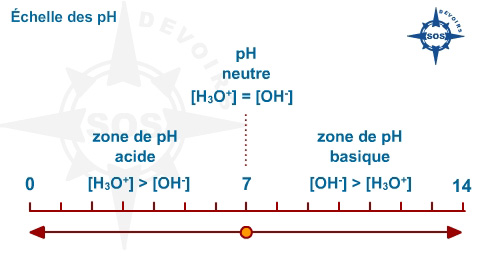
\includegraphics[scale=0.5]{echelle_ph.jpg}
\end{figure}

Schéma général d'une réaction acide-base: $\ce{Acide 1 + Base 2 <=> Base_{conj}1 + Acide_{conj}2}$

$$\kc=\frac{K_{a1}}{K_{a2}}$$

\subsection{Prévoir le sens d'évolution des réactions acide-base}

\begin{itemize}
\item[$\bullet$] Qualitativement: la réaction évolue préférentiellement dans le sens qui consomme l'acide et la base les plus forts et produits les plus faibles.
\item[$\bullet$] Quantitativement:
	\begin{itemize}
	\item Si $\kc>10^3$: réaction complète
	\item Si $\kc<10^{-3}$: réaction impossible
	\item Si $10^{-3}<\kc<10^3$: réaction équilibrée avec une évolution préférentielle de la réaction de la gauche vers la droite si $\kc>1$.
	\end{itemize}
\end{itemize}

\subsection{Prévoir les forces relatives des acides et des bases}

\paragraph{Cas des hydracides (H-A)}
La labilité d'un H, c'est-à-dire son aptitude à se séparer de la molécule HA sous forme de \ce{H+}, est liée à la polarité et à la force de la liaison H-A.
\begin{itemize}
\item[$\bullet$] Plus la liaison est \textbf{polaire}, plus l'acide est \textbf{fort} (effet prédominant pour les acides d'une même période).
	La polarité est liée à \textbf{l'électronégativité} de A mais aussi à la taille de l'ion \ce{A-}, les plus gros ions étant + stables.
\item[$\bullet$]Plus la liaison est \textbf{faible}, plus l'acide est \textbf{fort}
\end{itemize}

\paragraph{Cas des oxoacides (H-O-Z)}
L'acidité résulte de la polarité élevée de la liaison O-H.
\begin{itemize}
\item[$\bullet$] Plus le nombre d'atomes \textbf{O} liés à l'atome central est grand, plus l'acide est \textbf{fort}
\item[$\bullet$] Pour un même nombre d'atomes O liés à l'atome central, plus \textbf{l'électronégativité} de l'atome central est élevé plus l'acide est \textbf{fort}
\end{itemize}

\section{Définition des acides et des bases selon Lewis}
Un acide est un accepteur de doublet (il possède une orbitale libre) et une base est un donneur de doublet (elle possède un doublet libre).
En donnant son doublet libre la base forme une liaison covalente dative avec l'acide.

Les acides et les bases au sens d'Arrhénius et de Brönsted sont des acides et des bases au sens de Lewis.

\section{pH des acides et des bases en solution aqueuse}

Hypothèse: on néglige les ions \ce{H3O+} provenant de l'autoprotolyse de l'eau (formules dans formulaire).

\renewcommand{\arraystretch}{1.5}
\begin{tabular}{|>{\bf}c|c|}
	\hline
	Acide Fort & $pH=-\log{C_0}$ \\
	\hline
	Base Forte & $pH=14+\log{C_0}$ \\
	\hline
	Acide faible & $pH=\frac{1}{2}pK_a-\frac{1}{2}\log{C_0}$ \\
	\hline
	Base faible & $pH=7+\frac{1}{2}pK_a+\frac{1}{2}\log{C_0}$ \\
	\hline
	Sel acide & $pH=\frac{1}{2}pK_a-\frac{1}{2}\log{C_0}$ \\
	\hline
	Sel basique & $pH=7+\frac{1}{2}pK_a+\frac{1}{2}\log{C_0}$ \\
	\hline
\end{tabular}

\vspace{1cm}

\begin{itemize}

\item[$\bullet$] Degré d'ionisation des acides faibles: $D.I.=\frac{[A^{-}]}{C_0(HA)}\times 100\%$.
	Un faible degré d'ionisation signifie que le soluté est constitué essentiellement de molécules de HA.

\item[$\bullet$] Degré de protonisation des bases faibles: $D.P.=\frac{[\ce{BH+}]}{C_0(B)}\times 100\%$

\item[$\bullet$] Sels acides: sels résultant de la réaction d'un acide fort avec une base faible (ex: \ce{HCl(aq) + NH+(aq) -> NH4Cl(aq)}).
	Comme le sel est un électrolyte fort, il se dissocie totalement dans la solution aqueuse.

\item[$\bullet$] Sels basiques: sels résultant de la réaction d'un acide faible et d'une base forte (ex: \ce{CH3COOH(aq) + NaOH(aq) -> CH3COONa(aq) + H2O(l)})

\item[$\bullet$] Sels neutres: sels résultant de la réaction d'un acide fort et d'une base forte.
	Ex: \ce{HCl(aq) + KOH(aq) -> KCl(aq) + H2O(l)}: ni \ce{K+} ni \ce{Cl-} ne réagissent avec l'eau car HCl (acide fort) et KOH (base forte) n'existent pas en solution aqueuse.
\end{itemize}



\subsection{pH des solutions tampons}
Une solution tampon est constituée à la fois d'un acide faible et de sa base conjuguée ou d'une base faible et de son acide conjugué.
Les tampons stabilisent le pH d'une solution en fournissant une source ou un piège à protons.
$$pH = pK_a + \log{\frac{C_0(base)}{C_0(acide)}}$$

Pour utiliser cette formule, il faut que le $K_a$ soit relativement faible et que
$$0.1<\frac{C_{sel}}{C_{acide}}<10$$
car on fait comme hypothèses que $\ce{[CH3COOH]}=C_{acide}$ et [\ce{CH3COO-}]=$C_{sel}$
[Exercices slide 38]

\subsection{Résumé}
Acide Fort +
\begin{itemize}
\item[$\bullet$] Base Forte:
	\begin{itemize}
	\item si excès d'acide $\rightarrow$ AF
	\item si équivalence $\rightarrow$ sel neutre
	\item si excès de base $\rightarrow$ BF
	\end{itemize}
\item[$\bullet$] acide faible $\rightarrow$ A.F. dilué
\item[$\bullet$] base faible:
	\begin{itemize}
	\item si excès d'AF $\rightarrow$ AF dilué
	\item si équivalence $\rightarrow$ sel acide
	\item si excès bf $\rightarrow$ mélange tampon
	\end{itemize}
\item[$\bullet$] sel acide $\rightarrow$ AF dilué
\item[$\bullet$] sel neutre $\rightarrow$ AF dilué
\item[$\bullet$] sel basique:
	\begin{itemize}
	\item si excès sel $\rightarrow$ mélange tampon
	\item si équivalence $\rightarrow$ af
	\item si excès AF $\rightarrow$ AF dilué
	\end{itemize}
\item[$\bullet$] mélange tampon bf et son sel:
	\begin{itemize}
	\item si excès AF $\rightarrow$ AF dilué
	\item si équivalence $\rightarrow$ sel acide
	\item si excès bf $\rightarrow$ mélange tampon
	\end{itemize}
\item[$\bullet$] tampon af et son sel
	\begin{itemize}
	\item si excès AF $\rightarrow$ AF dilué
	\item si équivalence $\rightarrow$ af
	\item si excès af $\rightarrow$ mélange tampon
	\end{itemize}
\end{itemize}
(Même principe pour les Bases Fortes)

acide faible +
\begin{itemize}
\item[$\bullet$] sel neutre $\rightarrow$ af dilué
\item[$\bullet$] sel basique de l'af et BF $\rightarrow$ mélange tampon
\end{itemize}

base faible + sel acide de la bf et AF $\rightarrow$ mélange tampon

\section{Titrages acido-basiques}
Un titrage permet de déterminer les concentrations d'une solution inconnue à partir d'une solution de concentration connue.

Le point d'équivalence est le moment où $n_{\ce{OH-}} = n_{\ce{H3O+}}$ (mais pH$\neq 7$ \emph{sauf si} acide fort et base forte).
Pour le détecter $\rightarrow$ indicateur (acide ou base faible) qui change de couleur selon sa forme ionisée.

\subsection{Neutralisation d'un acide fort (HCl) par une base forte (NaOH)}

\begin{figure}[ht!]
\centering
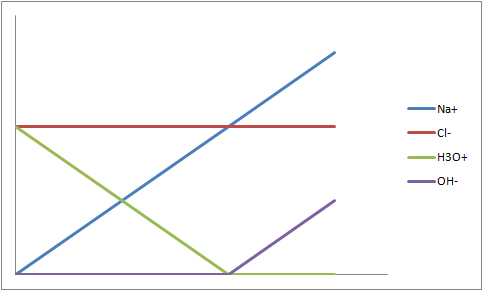
\includegraphics[scale=0.7]{DiagBilanAFBF.png}
\caption{Diagramme bilan}
\end{figure}

\part{Annexes}

\section{Notations}
De nombreuses notations seront utilisées au cours de cette synthèse.
Pour des raisons de concision, leur signification ne sera pas rappelée à chaque fois mais elle sera indiqué dans la Table~\ref{tab:notations}.
\begin{table}[h!]
	\begin{center}
		\begin{tabular}{ll}
			$\nu$ & La fréquence d'un rayonnement électromagnétique\\
			$\lambda$ & La longeur d'onde d'un rayonnement électromagnétique\\
			$c$ & La vitesse d'un rayonnement électromagnétique\\
			$c_0$ & La vitesse de la lumière\\
			$h$ & La constante de Planck\\
			$E_A$ & \'Electroaffinité d'un atome, voir section~\ref{sec:electro} page~\pageref{sec:electro}\\
			$E_I$ & \'Energie d'ionisation d'un atome, voir section~\ref{sec:ioni} page~\pageref{sec:ioni}\\
			$E_l$ & \'Energie de liaison, voir section~\ref{sec:E_l} page~\pageref{sec:E_l}\\ % FIXME: E_l ou E_D ?
			$E_N$ & \'Energie de neutralisation entre deux atomes\\
			$N_A$ & Nombre d'avogadro\\
			%$r$ & Le rayon d'un atome\\
			$C_s$ & Capacité calorifique spécifique d'un corps, voir section~\ref{sec:C_s} page~\pageref{sec:C_s}\\
			$\ccal$ & Capacité calorifique d'un corps, voir section~\ref{sec:C_cal} page~\pageref{sec:C_cal}\\
			$\Delta H$ & Variation d'enthalpie, voir section~\ref{sec:DH} page~\pageref{sec:DH}
		\end{tabular}
		\label{tab:notations}
		\caption{Répertoire des notations}
	\end{center}
\end{table}

\end{document}
